%!TEX root = ../thesis.tex
\chapter{Related Work\label{ch:pastwork}}

This work is based on a number of previous research efforts. The samples are collected with an existing hardware device. And there also exist some efforts on recognition based on local features.

% include other files for sections of this chapter. These use the 'input' command since each section within a chapter should not start a new page.
% If you want to swap the order of sections, it is as simple as reversing the order you include them.
\section{Hardware}
\label{sec:pastwork:hardware}

% ~\cite{Li:2011ur,Li:2010en,Zhang:2009dp}

Different approaches are available for 3D imaging including laser scanning~\cite{Blais:1988te}, viewpoint reconstruction~\cite{Hartley:2000un} and structured light scanning~\cite{Halioua:1984ue}. Structured light scanning, compared to other approaches, is fast and accurate. For palmprint recognition, speed is an important factor. The verification or identification result must be given in a short time. Otherwise the system is barely suitable for real-world applications.

% http://en.wikipedia.org/wiki/Structured-light_3D_scanner

Projecting a narrow band of light onto a three-dimensionally shaped surface produces a line of illumination that appears distorted from other perspectives than that of the projector, and can be used for an exact geometric reconstruction of the surface shape (light section).

A faster and more versatile method is the projection of patterns consisting of many stripes at once, or of arbitrary fringes, as this allows for the acquisition of a multitude of samples simultaneously. Seen from different viewpoints, the pattern appears geometrically distorted due to the surface shape of the object.

\begin{figure}[htb]
  \begin{center}
    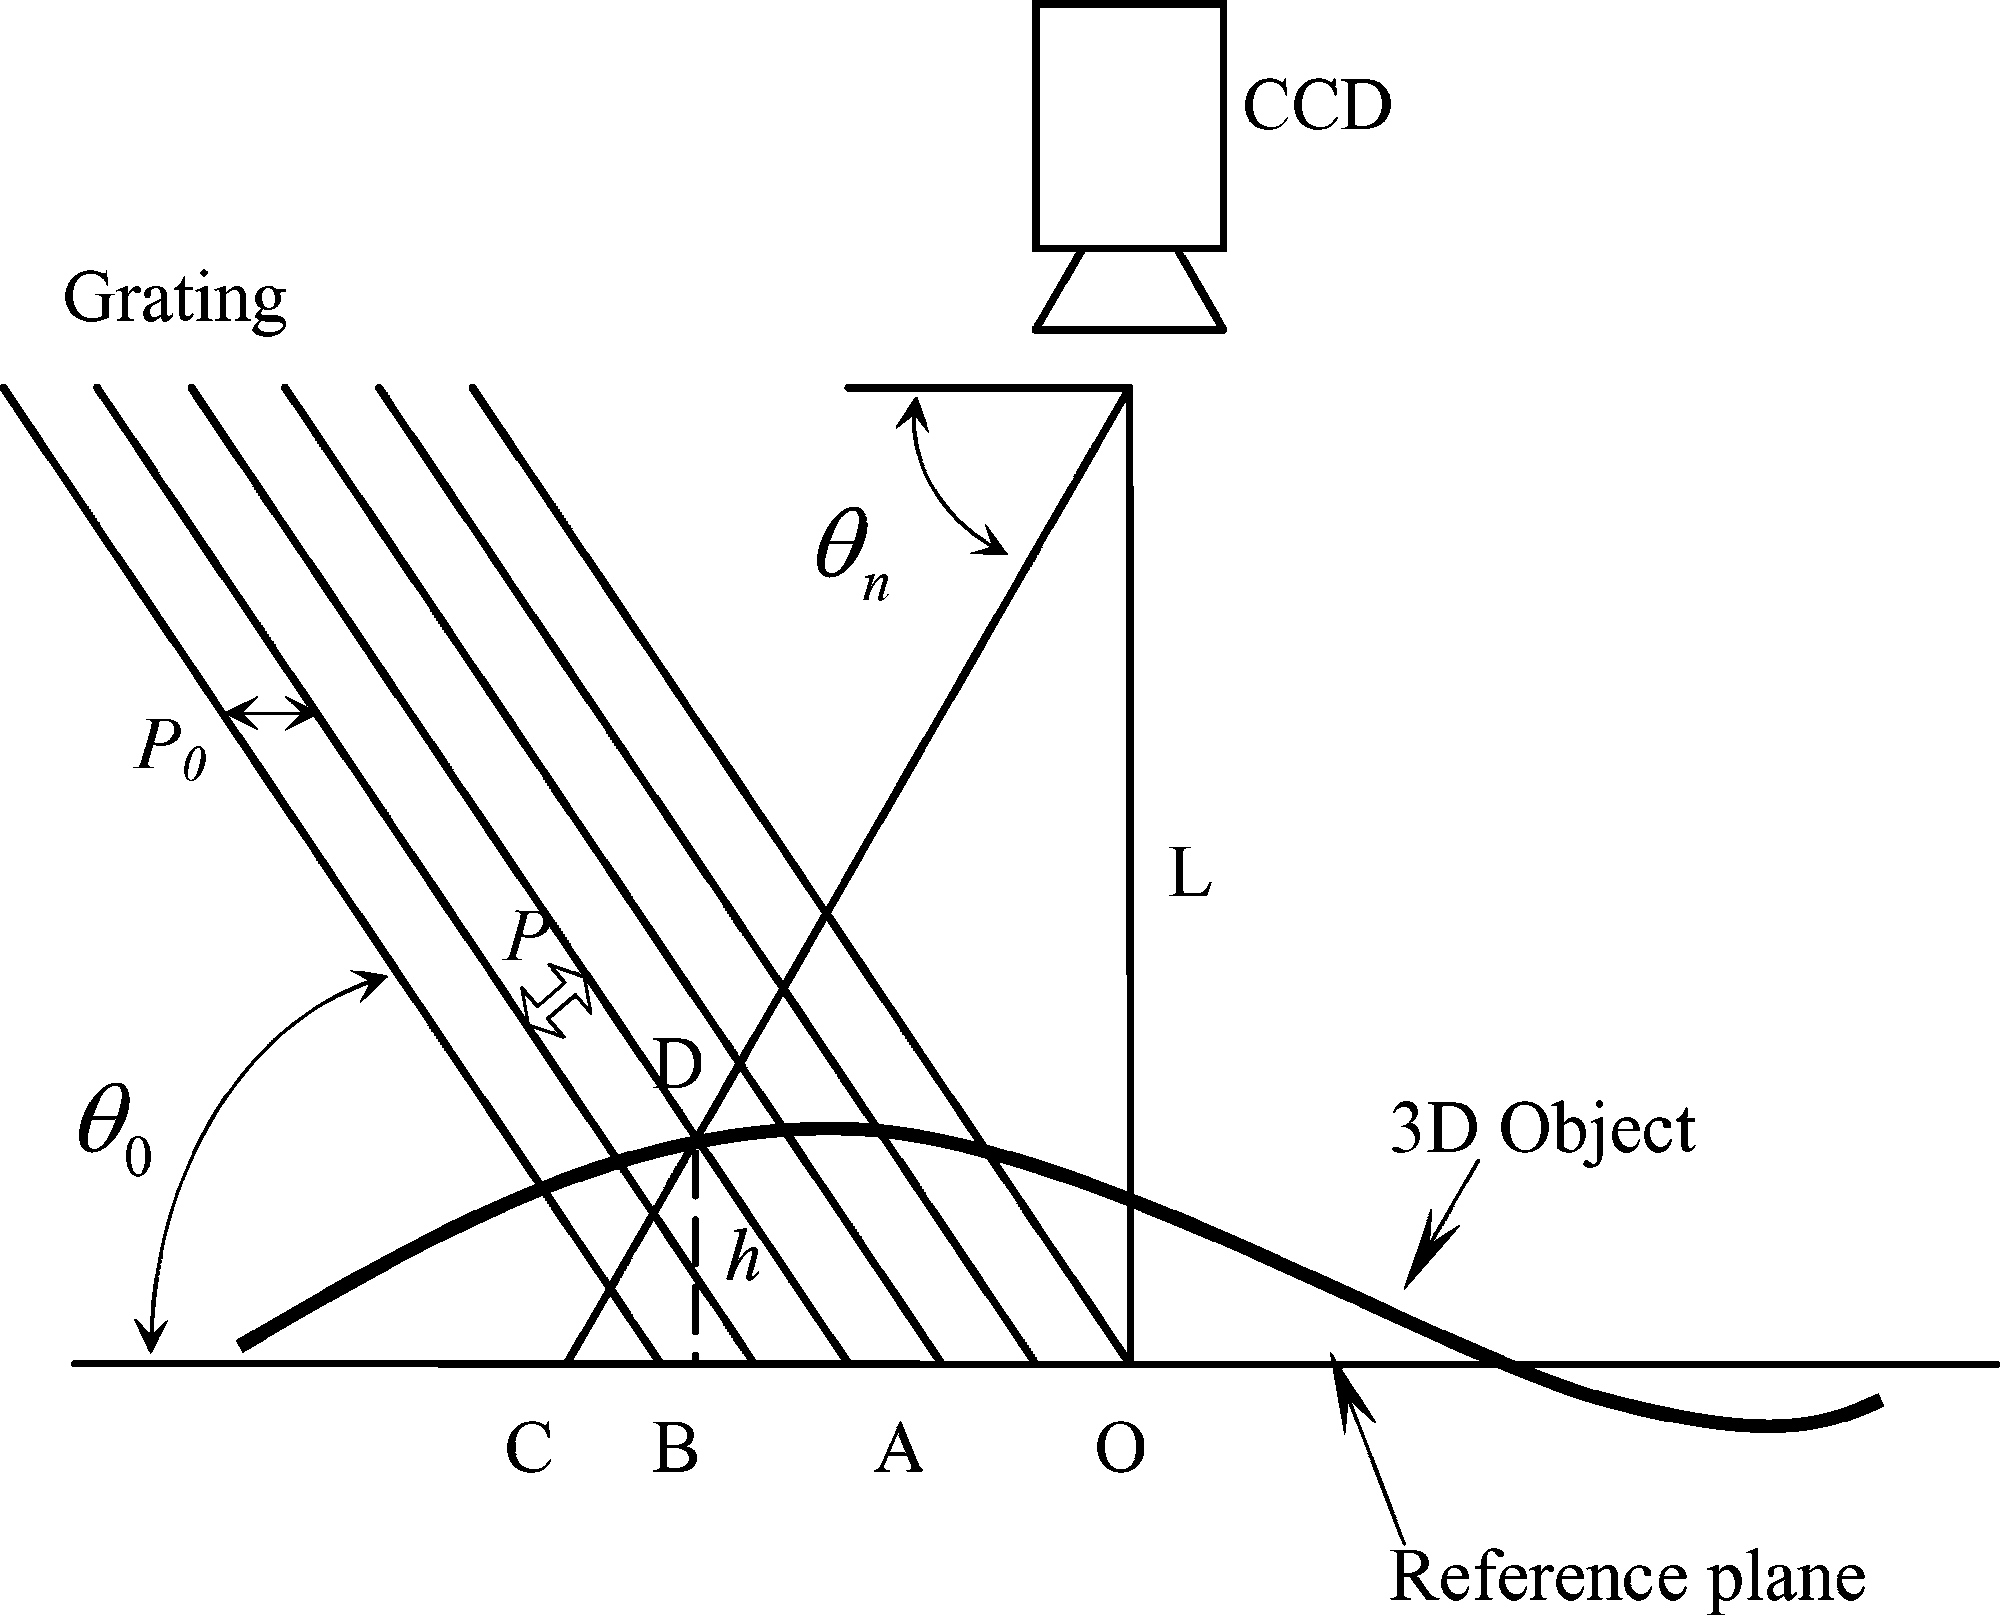
\includegraphics[width=0.9\linewidth]{ch-pastwork/figures/sli}
    \caption[The principle of structured-light imaging]{The principle of structured-light imaging\cite{Li:2009eq}}
    \label{fig:pastwork:sli}
  \end{center}
\end{figure}

Although many other variants of structured light projection are possible, patterns of parallel stripes are widely used. Figure~\ref{fig:pastwork:strippattern} shows the geometrical deformation of a strip pattern projected onto a palm. The displacement of the stripes allows for an exact retrieval of the 3D coordinates of any details on the palm's surface.

David et. al designed a 3D palmprint capturing device~\cite{Zhang:2008kc}. The system proposed has a resolution of 768x576.

\begin{figure}[htb]
  \begin{center}
    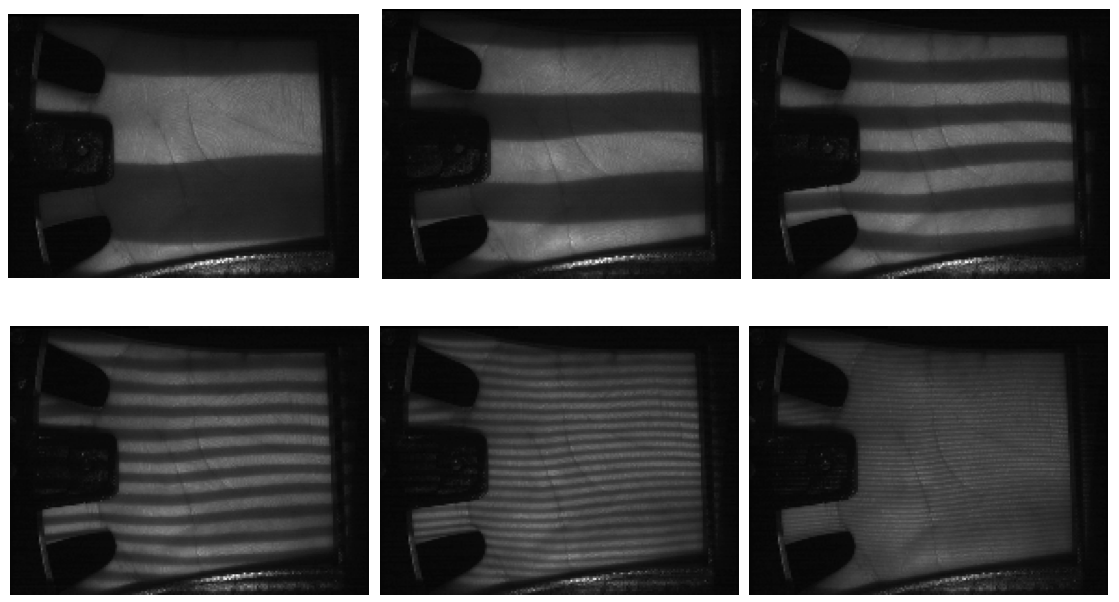
\includegraphics[width=0.9\linewidth]{ch-pastwork/figures/strippattern}
    \caption[Sample patterns of the stripes on the palm]{Sample patterns of the stripes on the palm~\cite{Li:2009eq}}
    \label{fig:pastwork:strippattern}
  \end{center}
\end{figure}

\section{Recognition Methods}
\label{sec:pastwork:recogmethods}

Traditionally, palmprint recognition has made use of either high or low resolution 2D palmprint images. High resolution images are suitable for forensic applications [3] while low resolution images are suitable for civil and commercial applications [4]. Most current research use low resolution palmprint recognition and is either texture-based or line-based. The texture-based methods include PalmCode [4], Competitive Code [5] and Ordinal Code [6]. These methods use a group of filters to enhance and extract the phase or directional features which can represent the texture of the palmprint. Line-based methods use line or edge detectors to explicitly extract line information from the palmprint that is then used for matching. The representative methods include Derivative of Gaussian based line extraction [7] and Modified Finite Radon transform (MFRAT) based line extraction [8].

In recent years, 3D techniques have been applied to biometric authentication, such as 3D face [9] and 3D ear recognition [10]. Most recently, a structured-light imaging [11, 12] 3D palmprint system [13] was developed that captures the depth information of a palmprint. This information is then used to calculate the Mean and the Gaussian curvatures for use in 3D palmprint matching and recognition. To date, however, there has been no work with 3D palmprints that has extracted global shape features, which may be useful in classification and indexing. For fingerprint, according to the global ridge structure and singularities, it can be classified into five classes: arch, tented arch, left loop, right loop and whorl [14]. Wu et al. classified the palmprint into six classes according to the palmprint principal lines [15]. Besides the exclusive classification technique, the continuous classification technique is also widely used for indexing the database for personal identification [16].

Some general features were extracted for recognition including 3D Mean Curvature Image, 3D Gauss Curvature Image and 3D Surface Type~\cite{Zhang:2008kc,Li:2009eq}.



